\hypertarget{_colorspace_8h}{
\section{Colorspace.h File Reference}
\label{_colorspace_8h}\index{Colorspace.h(114)@{Colorspace.h(114)}}
}


\subsection{Detailed Description}
Declaration of enumeration Colorspace. 



Definition in file \hyperlink{_colorspace_8h-source}{Colorspace.h}.

{\tt \#include $<$Magick++.h$>$}\par


Include dependency graph for Colorspace.h:\nopagebreak
\begin{figure}[H]
\begin{center}
\leavevmode
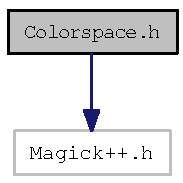
\includegraphics[width=62pt]{_colorspace_8h__incl}
\end{center}
\end{figure}


This graph shows which files directly or indirectly include this file:\nopagebreak
\begin{figure}[H]
\begin{center}
\leavevmode
\includegraphics[width=163pt]{_colorspace_8h__dep__incl}
\end{center}
\end{figure}
\subsection*{Enumerations}
\begin{CompactItemize}
\item 
enum \hyperlink{_colorspace_8h_7a7e24cdb2a27271343f0adceff89f65}{Colorspace} \{ \hyperlink{_colorspace_8h_7a7e24cdb2a27271343f0adceff89f657d1a82386f7d1d75c0891e466e77f980}{COLORSPACE\_\-GRAYSCALE}, 
\hyperlink{_colorspace_8h_7a7e24cdb2a27271343f0adceff89f657a29001c1d233a707de5354b40dbdad8}{COLORSPACE\_\-RGB}, 
\hyperlink{_colorspace_8h_7a7e24cdb2a27271343f0adceff89f65e6f46807495766afe46a6ed8f204804b}{COLORSPACE\_\-MONOCHROMATIC}, 
\hyperlink{_colorspace_8h_7a7e24cdb2a27271343f0adceff89f6561872e0836b51554b224e79e71e20ae7}{COLORSPACE\_\-UNDEFINED}
 \}
\begin{CompactList}\small\item\em Colorspace of an image. \item\end{CompactList}\end{CompactItemize}


\subsection{Enumeration Type Documentation}
\hypertarget{_colorspace_8h_7a7e24cdb2a27271343f0adceff89f65}{
\index{Colorspace.h@{Colorspace.h}!Colorspace@{Colorspace}}
\index{Colorspace@{Colorspace}!Colorspace.h@{Colorspace.h}}
\subsubsection[Colorspace]{\setlength{\rightskip}{0pt plus 5cm}enum {\bf Colorspace}}}
\label{_colorspace_8h_7a7e24cdb2a27271343f0adceff89f65}


Colorspace of an image. 

This enumeration represents the different colorspaces that an image may have. This enumeration depends internally on Magick++ image types implementation (see \href{http://www.imagemagick.org/Magick++/Enumerations.html#ImageType}{\tt ImageType on Magick++ documentation}). Only three choices are given, though there are many options available in Magick++.

\begin{Desc}
\item[Author:]Eliezer Talón (\href{mailto:elitalon@gmail.com}{\tt elitalon@gmail.com}) \end{Desc}
\begin{Desc}
\item[Date:]2008-09-25 \end{Desc}
\begin{Desc}
\item[Enumerator: ]\par
\begin{description}
\index{COLORSPACE\_\-GRAYSCALE@{COLORSPACE\_\-GRAYSCALE}!Colorspace.h@{Colorspace.h}}\index{Colorspace.h@{Colorspace.h}!COLORSPACE\_\-GRAYSCALE@{COLORSPACE\_\-GRAYSCALE}}\item[{\em 
\hypertarget{_colorspace_8h_7a7e24cdb2a27271343f0adceff89f657d1a82386f7d1d75c0891e466e77f980}{
COLORSPACE\_\-GRAYSCALE}
\label{_colorspace_8h_7a7e24cdb2a27271343f0adceff89f657d1a82386f7d1d75c0891e466e77f980}
}]A grayscale colorspace. \index{COLORSPACE\_\-RGB@{COLORSPACE\_\-RGB}!Colorspace.h@{Colorspace.h}}\index{Colorspace.h@{Colorspace.h}!COLORSPACE\_\-RGB@{COLORSPACE\_\-RGB}}\item[{\em 
\hypertarget{_colorspace_8h_7a7e24cdb2a27271343f0adceff89f657a29001c1d233a707de5354b40dbdad8}{
COLORSPACE\_\-RGB}
\label{_colorspace_8h_7a7e24cdb2a27271343f0adceff89f657a29001c1d233a707de5354b40dbdad8}
}]A RGB colorspace. \index{COLORSPACE\_\-MONOCHROMATIC@{COLORSPACE\_\-MONOCHROMATIC}!Colorspace.h@{Colorspace.h}}\index{Colorspace.h@{Colorspace.h}!COLORSPACE\_\-MONOCHROMATIC@{COLORSPACE\_\-MONOCHROMATIC}}\item[{\em 
\hypertarget{_colorspace_8h_7a7e24cdb2a27271343f0adceff89f65e6f46807495766afe46a6ed8f204804b}{
COLORSPACE\_\-MONOCHROMATIC}
\label{_colorspace_8h_7a7e24cdb2a27271343f0adceff89f65e6f46807495766afe46a6ed8f204804b}
}]A monochromatic colorspace. \index{COLORSPACE\_\-UNDEFINED@{COLORSPACE\_\-UNDEFINED}!Colorspace.h@{Colorspace.h}}\index{Colorspace.h@{Colorspace.h}!COLORSPACE\_\-UNDEFINED@{COLORSPACE\_\-UNDEFINED}}\item[{\em 
\hypertarget{_colorspace_8h_7a7e24cdb2a27271343f0adceff89f6561872e0836b51554b224e79e71e20ae7}{
COLORSPACE\_\-UNDEFINED}
\label{_colorspace_8h_7a7e24cdb2a27271343f0adceff89f6561872e0836b51554b224e79e71e20ae7}
}]An undefined colorspace. \end{description}
\end{Desc}



Definition at line 23 of file Colorspace.h.